% !TEX encoding = UTF-8 Unicode

\documentclass[a4paper,12pt]{report}

%--------------------------------------------------------------------------------------------------------------------------------------------------
%----------------------------------------------------------------Preamble-----------------------------------------------------------------------
%--------------------------------------------------------------------------------------------------------------------------------------------------

\usepackage[top=2.5cm, bottom=2.5cm, left=3.5cm, right=2.5cm]{geometry}

\usepackage{graphicx}
\usepackage[turkish]{babel}

\usepackage{longtable}
\usepackage{multirow}
\usepackage{thmtools}
\usepackage{hyperref}
\usepackage{amssymb}
\usepackage{amsmath}
\usepackage{mathtools}
\usepackage{xfrac} 

\usepackage{caption,setspace}

\usepackage{pdflscape}
\usepackage{pdfpages}

\usepackage{cite}
\usepackage{multirow}

\usepackage{setspace}
\usepackage{parskip}
\usepackage{enumitem}

\usepackage{titlesec}
\usepackage{titletoc}

\usepackage{appendix}

\usepackage{notoccite}
\usepackage{soul}

\usepackage{fontspec}
\setmainfont{Calibri}

  \declaretheorem{definition}
  \declaretheorem{theorem}
  \declaretheorem{proof}
  \declaretheorem{hypothesis}


\captionsetup[table]{name=Çizelge}
\captionsetup[table]{labelsep=space}
\captionsetup[figure]{labelsep=space}

  \setlength{\parskip}{6pt plus 1pt minus 1pt}


  \titleformat{\chapter}[display]
  {\bfseries\large}
  {\filleft\MakeUppercase{\chaptertitlename} \large\thechapter}
  {2ex}
  {\titlerule\vspace{2ex}\filleft}

  \titleformat{name=\chapter,numberless}[display]
  {\bfseries\large}
  {\titlerule}
  {-9ex}
  {\filleft\MakeUppercase}[\vspace{5ex}] \titlespacing*{\chapter}{0pt}{55pt}{6pt}

  \titleformat{\section}{\normalfont\normalsize\bfseries}{\thesection}{6pt}{}
  \titleformat{\subsection}{\normalfont\normalsize\bfseries}{\thesubsection}{6pt}{}
  \titleformat{\subsubsection}{\normalfont\normalsize\bfseries}{\thesubsubsection}{6pt}{}
  \setcounter{secnumdepth}{3}
  \setcounter{tocdepth}{3}

\setlist[itemize]{leftmargin=*}
\setlist[itemize]{labelsep=1.8em}
\setlist[enumerate]{leftmargin=*}
\setlist[enumerate]{labelsep=1.8em}

  \titlecontents{chapter}
  [0ex]
  {\addvspace{2ex}}
  {\MakeUppercase\@chapapp\ \thecontentslabel\quad \\}
  {\hspace{-0ex}}
  {\leaders\hbox{\normalfont$\m@th\mkern \@dotsep mu\hbox{.}\mkern \@dotsep mu$}\hfill\contentspage}
  [\addvspace{0pt}]

  \g@addto@macro\appendices{%
    \addtocontents{toc}{\protect\renewcommand{\protect\@chapapp}{\appendixname}}%
  }


  \newcommand\tocheading{\vspace{-3ex}\hfill Sayfa}
  \newcommand\lofheading{\vspace{-3ex}\hfill Sayfa}
  \newcommand\lotheading{\vspace{-3ex}\hfill Sayfa}

\dottedcontents{listoffigures}[3.8em]{}{2.3em}{1pc}

%--------------------------------------------------------------------------------------------------------------------------------------------------
%---------------------------------------------------Single spacing the lot and lof-------------------------------------------------------
%--------------------------------------------------------------------------------------------------------------------------------------------------
\makeatletter
\def\@chapter[#1]#2{\ifnum \c@secnumdepth >\m@ne
                       \if@mainmatter
                         \refstepcounter{chapter}%
                         \typeout{\@chapapp\space\thechapter.}%
                         \addcontentsline{toc}{chapter}%
                                   {\protect\numberline{\thechapter}#1}%
                       \else
                         \addcontentsline{toc}{chapter}{#1}%
                       \fi
                    \else
                      \addcontentsline{toc}{chapter}{#1}%
                    \fi
                    \chaptermark{#1}%
                    \if@twocolumn
                      \@topnewpage[\@makechapterhead{#2}]%
                    \else
                      \@makechapterhead{#2}%
                      \@afterheading
                    \fi}

\renewcommand{\@biblabel}[1]{[#1]\hfill\hspace{12pt}}

\makeatother

\begin{document}

\shorthandoff{=}% Türkçe yazım için geçerli
\newgeometry{top=3cm, bottom=0cm}
\shorthandon{=}
\begin{titlepage}
\begin{center}
\begin{singlespacing}
\large T.C. \\ YILDIZ TEKNİK ÜNİVERSİTESİ\\FEN BİLİMLERİ ENSTİTÜSÜ\\[4cm]
\large TEZ BAŞLIĞI\\[5cm]
\large ADINIZ SOYADINIZ\\[3cm]
\large DOKTORA TEZİ\\BİLGİSAYAR MÜHENDİSLİĞİ ANABİLİM DALI\\BİLGİSAYAR MÜHENDİSLİĞİ PROGRAMI\\[3cm] 
\large DANIŞMAN\\ DANIŞMANINIZIN ADI\\[2cm]
\large İSTANBUL, 2018
\end{singlespacing}
\end{center}
\end{titlepage}
\restoregeometry
\begin{titlepage}
\begin{center}
\bfseries\large T.C. \\ YILDIZ TEKNİK ÜNİVERSİTESİ\\ FEN BİLİMLERİ ENSTİTÜSÜ\\[1.5cm]
\bfseries\large TEZ BAŞLIĞI\\[1.5cm]
\end{center}
\begin{singlespacing}
\textnormal{Adınız SOYADINIZ tarafından hazırlanan tez çalışması 01.01.2018 tarihinde aşağıdaki jüri tarafından Yıldız Teknik Üniversitesi Fen Bilimleri Enstitüsü Bilgisayar Mühendisliği Anabilim Dalı'nda \textbf{DOKTORA TEZİ} olarak kabul edilmiştir.}\\[1cm] 
\textbf{Tez Danışmanı}\\
\textnormal{Prof. Dr. Abc DEF\\ Yıldız Teknik Üniversitesi}\\[1cm]
\textbf{Jüri Üyeleri}\\

\textnormal{Prof. Dr. Abc DEF}\\
\textnormal{Yıldız Teknik Üniversitesi} \hfill \rule{5cm}{1pt}\\[1cm]

%Jüri satırlarını gerektiği kadar arttırmayı unutmayın!

\end{singlespacing}
\end{titlepage}

\begin{titlepage}
\shorthandoff{=}
\topmargin=80pt
\shorthandon{=}
\begin{flushright}
\uppercase{\bfseries{\large önsöz}}\\[0.5cm]
\hrule
\vspace{2ex}%
\end{flushright}
\begin{singlespacing}
Önsöz buraya gelecek
\\
\\
Ocak, 2018
\\
\\
Adınız SOYADINIZ

\end{singlespacing}
\end{titlepage}

%--------------------------------------------------------------------------------------------------------------------------------------------------
%------------------------------NORMAL SAYILI SAYFALAR--------------------------
%--------------------------------------------------------------------------------------------------------------------------------------------------


\renewcommand{\contentsname}{İÇ\.{I}NDEK\.{I}LER} %İçindekiler başlığının düzenlenmesi

\renewcommand\chaptername{BÖLÜM}
\renewcommand\appendixname{EK}

\pagenumbering{roman}
\setcounter{page}{4}
\tableofcontents
\addtocontents{toc}{\tocheading}

\renewcommand*{\textoverline}[1]{$\overline{\hbox{#1}}$}

\chapter*{SİMGE LİSTESİ}
\vspace{-2pt}
\addcontentsline{toc}{chapter}{SİMGE LİSTESİ}
\begin{table}[h]
	\begin{tabular}{p{2cm} l}
		k & Komşuluk sayısı \\
		\texorpdfstring{M\textsubscript{S}}{} & S alt kümesinin faydası \\
		\texorpdfstring{r\textsubscript{\textoverline{cf}}}{} & Özellik-sınıflandırma korelasyonlarının ortalama değeri \\
		\texorpdfstring{r\textsubscript{\textoverline{ff}}}{} & Özellik-özellik korelasyonlarının ortalama değeri \\
		\texorpdfstring{R\textsubscript{i}}{} & i. kümedeki sıralama değerlerinin toplamı \\
	\end{tabular}
\end{table}


\chapter*{KISALTMA LİSTESİ}
\vspace{-2pt}
\addcontentsline{toc}{chapter}{KISALTMA LİSTESİ}
\begin{longtable}[l]{p{2cm} l}

AST &Abstract Syntax Tree \\
YSA &Yapay Sinir Ağları \\
XML &eXtensible Markup Language \\

\end{longtable}

  \renewcommand{\listfigurename}{ŞEK\.{I}L L\.{I}STES\.{I}}
  \renewcommand{\listtablename}{Ç\.{I}ZELGE L\.{I}STES\.{I}}
  \renewcommand{\turkishtablename}{Çizelge}

{%
\let\oldnumberline\numberline%
\renewcommand{\numberline}{\figurename~\oldnumberline}%
\addcontentsline{toc}{chapter}{\listfigurename}
\listoffigures%
\addtocontents{lof}{\lofheading}
}

{%
\let\oldnumberline\numberline%
\renewcommand{\numberline}{\tablename~\oldnumberline}%
\addcontentsline{toc}{chapter}{\listtablename}
\listoftables%
\addtocontents{lot}{\lotheading}
}


\chapter*{\"{O}ZET}
\vspace{-12pt}
\begin{center}
\large{\bfseries{TEZ BAŞLIĞI}}\\[1cm]

\fontsize{12pt}{12pt}\selectfont
Adınız SOYADINIZ\\[1cm]

Bilgisayar Mühendisliği Anabilim Dalı\\[6pt]
Doktora Tezi\\[1cm]

Tez Danışmanı: Prof. Dr. Abc DEF\\[1cm]

\end{center}

\begin{singlespacing}
Lorem ipsum dolor sit amet, consectetur adipiscing elit. Nulla sit amet pretium metus. Etiam maximus neque velit, id euismod elit lobortis sed. Phasellus id sem volutpat, volutpat nulla id, tempus lorem. In eros massa, vestibulum ut hendrerit gravida, molestie eget est. Vestibulum ac nulla at nunc fermentum faucibus. Curabitur rutrum est a ex suscipit, eget sodales massa pulvinar. Fusce vitae mi magna. Curabitur ut gravida nulla. Ut tristique efficitur rutrum.
\\
\\
\textbf{Anahtar Kelimeler:} Anahtar kelimeler
\end{singlespacing}
\vfill
\vspace{1ex}
\hrule
\begin{flushright}
\textbf{YILDIZ TEKNIK ÜNİVERSİTESİ FEN BİLİMLERİ ENSTİTÜSÜ}
\end{flushright}

\chapter*{ABSTRACT}
\vspace{-12pt}
\begin{center}
\large{\bfseries{İNGİLİZCE TEZ BAŞLIĞI}}\\[1cm]

\fontsize{12pt}{12pt}\selectfont
Adınız SOYADINIZ\\[1cm]

Department of Computer Engineering\\[6pt]
PhD. Thesis\\[1cm]

Advisor: Prof. Dr. Abc DEF\\[1cm]
\end{center}

\begin{singlespacing}
Lorem ipsum dolor sit amet, consectetur adipiscing elit. Nulla sit amet pretium metus. Etiam maximus neque velit, id euismod elit lobortis sed. Phasellus id sem volutpat, volutpat nulla id, tempus lorem. In eros massa, vestibulum ut hendrerit gravida, molestie eget est. Vestibulum ac nulla at nunc fermentum faucibus. Curabitur rutrum est a ex suscipit, eget sodales massa pulvinar. Fusce vitae mi magna. Curabitur ut gravida nulla. Ut tristique efficitur rutrum.
\\
\\
\textbf{Keywords:} İngilizce anahtar kelimeler
\end{singlespacing}

\vfill
\hrule
\begin{flushright}
\textbf{YILDIZ TECHNICAL UNIVERSITY \\ GRADUATE SCHOOL OF NATURAL AND APPLIED SCIENCES}
\end{flushright}


%--------------------------------------------------------------------------------------------------------------------------------------------------
%-------------------------------------------ANA METİN------------------------------------------------------------------
%--------------------------------------------------------------------------------------------------------------------------------------------------

\onehalfspacing


\chapter{GİRİŞ} %BU BÖLÜMÜN ADINI DEĞİŞTİRMEYİN. FBE TARAFINDAN İSTENİLEN ZORUNLU BAŞLIKTIR

\pagenumbering{arabic}

Lorem ipsum dolor sit amet, consectetur adipiscing elit. Curabitur et egestas magna. Etiam dolor velit, convallis in iaculis quis, tincidunt sit amet diam. Donec rhoncus pulvinar odio in mattis. Nullam leo risus, tincidunt non dignissim vel, ultrices vitae est. Proin ut augue elit. Nunc feugiat interdum metus sed blandit. Curabitur at venenatis elit, pellentesque ullamcorper augue.
\par
Sed porta iaculis ipsum, gravida aliquet metus tristique fringilla. Donec lobortis metus vitae aliquet luctus. Suspendisse potenti. In eleifend, elit eget laoreet viverra, mauris ante aliquam tortor, id luctus eros massa quis lorem. Donec neque orci, efficitur et cursus vel, volutpat a nulla. Aliquam faucibus faucibus eros, vitae vestibulum nunc ornare eget. Duis sed turpis eget augue fringilla blandit id ut nisl.

\section{Literatür Özeti} %BU BÖLÜMÜN ADINI DEĞİŞTİRMEYİN. FBE TARAFINDAN İSTENİLEN ZORUNLU BAŞLIKTIR
\label{sec: literatur ozeti}
Lorem ipsum dolor sit amet, consectetur adipiscing elit. Integer malesuada est eget ligula tempor, quis aliquam ligula tempus. Pellentesque quam eros, tristique non tincidunt a, tristique nec nibh. Quisque a purus congue, facilisis velit ut, malesuada est. Suspendisse eget euismod leo, ut rhoncus urna. Sed in arcu libero. Proin id cursus mauris. Duis mi mauris, aliquam et nibh eget, elementum porta ipsum. Nullam et vestibulum mi. Donec vulputate interdum orci quis auctor. Sed eleifend libero faucibus dolor sagittis, quis ullamcorper augue fermentum. Morbi scelerisque enim sit amet tempor volutpat. Phasellus imperdiet purus libero, vitae elementum quam interdum vel. Phasellus convallis velit ac risus condimentum, sit amet imperdiet lorem maximus. Sed egestas mattis semper. Fusce viverra fringilla nulla, et dictum elit. Fusce mollis a nisi ut luctus.

\section{Tezin Amacı} %BU BÖLÜMÜN ADINI DEĞİŞTİRMEYİN. FBE TARAFINDAN İSTENİLEN ZORUNLU BAŞLIKTIR
\label{sec: amaç}
Lorem ipsum dolor sit amet, consectetur adipiscing elit. Integer malesuada est eget ligula tempor, quis aliquam ligula tempus. Pellentesque quam eros, tristique non tincidunt a, tristique nec nibh. Quisque a purus congue, facilisis velit ut, malesuada est. Suspendisse eget euismod leo, ut rhoncus urna. Sed in arcu libero. Proin id cursus mauris. Duis mi mauris, aliquam et nibh eget, elementum porta ipsum. Nullam et vestibulum mi. Donec vulputate interdum orci quis auctor. Sed eleifend libero faucibus dolor sagittis, quis ullamcorper augue fermentum. Morbi scelerisque enim sit amet tempor volutpat. Phasellus imperdiet purus libero, vitae elementum quam interdum vel. Phasellus convallis velit ac risus condimentum, sit amet imperdiet lorem maximus. Sed egestas mattis semper. Fusce viverra fringilla nulla, et dictum elit. Fusce mollis a nisi ut luctus.

\section{Orijinal Katkı} %FBE TARAFINDAN İSTENİLEN ZORUNLU BAŞLIKTIR. BU BAŞLIĞI AŞAĞIDAKİ 2 SENEÇEKTEN SİZE UYGUN OLANLA DEĞİŞTİREBİLİRSİNİZ
		%   1. "Orijinal Katkı"
                %     2. "Hipotez"
\label{sec:original}

Lorem ipsum dolor sit amet, consectetur adipiscing elit. Maecenas erat quam, fermentum non enim at, malesuada bibendum lorem. Proin convallis massa eget mauris volutpat, at tincidunt nisi luctus. Suspendisse ultricies finibus risus, ac suscipit sem posuere sed \cite{ref1}, \cite{ref2}, \cite{ref3}. Ut vel convallis ligula. Maecenas bibendum purus id aliquet pretium. Nam felis ipsum, consectetur vitae odio eu, ullamcorper porta dolor. Nam aliquam urna vitae nulla elementum, eget tempor diam tincidunt. Suspendisse et dolor ex. Nunc vel leo et nibh iaculis cursus. Nullam tristique ullamcorper leo vel porttitor. Pellentesque habitant morbi tristique senectus et netus et malesuada fames ac turpis egestas. Nulla interdum dapibus ante venenatis ultricies. In viverra ornare pharetra. Aenean ornare vestibulum rhoncus. Ut luctus lacus a enim viverra, et luctus orci condimentum. Phasellus ultrices augue at commodo condimentum.


\par
Sed quis malesuada dui. Praesent imperdiet suscipit neque nec fringilla. Nullam laoreet posuere diam, ac pretium lorem. Duis porta rhoncus velit, non imperdiet ex convallis quis. Nulla et nulla ultricies, rhoncus urna eget, tincidunt orci. Mauris bibendum, lectus vel laoreet mollis, dolor diam tristique nisi, nec ornare libero lectus eu purus. Nunc metus lorem, hendrerit ac elit sed, iaculis maximus nisi. Aenean varius, lectus mollis ornare imperdiet, magna lacus hendrerit libero, vitae tristique mauris urna vitae erat.

\par
Fusce ac nibh auctor, feugiat sem quis, interdum augue \cite{ref4}. Ut sed risus ut justo blandit pretium sed sed purus. Donec auctor, ex a laoreet convallis, quam ex lacinia enim, sit amet scelerisque felis tortor in risus. Morbi viverra congue ultrices. Nullam molestie sagittis nisl, eget rhoncus nunc congue a. Curabitur accumsan urna ut diam pretium tempor. Aenean at turpis sed nisl posuere imperdiet.

\begin{table}[h]
\centering
\caption{Çizelge başlığı}
\label{tab:label}
\begin{tabular}{|l|l|}
\hline
 Abcd     & Abcd           \\ \hline
Abcd     & Abcd           \\
              & Abcd  \\
              & Abcd          \\ \hline
\end{tabular}

\end{table}

\par
Maecenas feugiat porttitor tellus volutpat sodales. Sed pulvinar ex vel nisi ultrices, quis rhoncus tortor facilisis. Praesent a fringilla neque. Duis diam sem, faucibus egestas ex at, eleifend dictum risus. Nulla pulvinar pharetra dapibus. Nunc at \cite{ref5} scelerisque nisl, at sodales orci. Morbi at ex lectus. Maecenas sed pretium mi. In id metus arcu. Donec nec lobortis eros. Nulla vitae mi varius, imperdiet nibh id, tincidunt nisl. Praesent felis augue, sodales id rutrum et, dictum at purus.

\shorthandoff{=}
\begin{figure}[h]
	\begin{center}
		\fbox{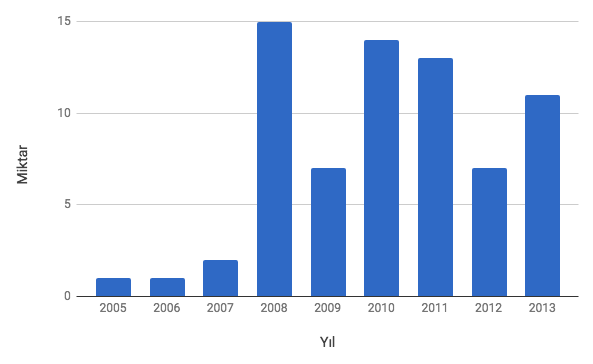
\includegraphics[width=12cm]{figures/example.png}}
	\end{center}
	\caption{Resim başlığı}
	\label{fig:label}
\end{figure}
\shorthandon{=}

\par
Aenean id tellus quis leo mollis efficitur. Morbi fermentum, nunc vel auctor semper, erat arcu porttitor orci, in faucibus sem dui sit amet libero. In sed varius nisl. Curabitur eget odio sit amet metus pulvinar placerat sed in est. Phasellus convallis nulla in mollis blandit \cite{ref6}. Lorem ipsum dolor sit amet, consectetur adipiscing elit. Integer scelerisque mattis eros, ut egestas felis convallis vel.



%--------------------------------------------------------------------------------------------------------------------------------------------------
%---------------------------------------------------------------Bibliography------------------------------------------------------------------
%!!!!!!!!!!!!!!!!!!
%BURAYI DEĞİŞTİRMEYİN!!! SADECE REFERENCES.BIB DOSYASINI DÜZENLEYİN. 
%!!!!!!!!!!!!!!!!
  \renewcommand{\bibname}{KAYNAKLAR} %Kaynakça başlığının düzenlenmesi

\begin{singlespacing}
\bibliography{references}{}
\bibliographystyle{ytu_fbe}
\addcontentsline{toc}{chapter}{KAYNAKLAR}
\end{singlespacing}
%--------------------------------------------------------------------------------------------------------------------------------------------------
%-------------------------------------EKLER-------------------------------------------------------------------
%--------------------------------------------------------------------------------------------------------------------------------------------------

\begin{appendices}
\chapter{EK ADI}
\label{app:metrics}
\onehalfspacing

Ekler bu kısma gelecek.

\end{appendices}

%--------------------------------------------------------------------------------------------------------------------------------------------------
%-----------------------------ÖZGEÇMİŞ---------------------------
%--------------------------------------------------------------------------------------------------------------------------------------------------
\chapter*{ÖZGEÇMİŞ}
\addcontentsline{toc}{chapter}{ÖZGEÇMİŞ}

\begin{table}[!h]
\begin{tabular}{l l}
\multicolumn{2}{l}{\bfseries{KİŞİSEL BİLGİLER}}\\[2ex]
\bfseries{Adı Soyadı} & : Adınız SOYADINIZ\\[2ex]
\bfseries{Doğum Tarihi ve Yeri} & : 01.01.2018 - İstanbul\\[2ex]
\bfseries{Yabancı Dili} & : İngilizce\\[2ex]
\bfseries{E-posta} & : example@example.com\\[5ex]
\end{tabular}

\begin{tabular}{l l l p{3cm}}
\multicolumn{4}{l}{\bfseries{ÖĞRENİM DURUMU}}\\[2ex]
\bfseries{Derece} & \bfseries{Alan} & \bfseries{Okul/üniversite} & \bfseries{Mezuniyet Yılı} \\[2ex]
Y. Lisans & Bilgisayar Müh. & Yıldız Teknik Üniversitesi & 2010 \\ [2ex]
Lisans & Bilgisayar Müh. & Yıldız Teknik Üniversitesi & 2008 \\[2ex]
Lise & Fen Bilimleri & Yıldız Teknik Lisesi & 2004 \\[2ex]
\end{tabular}

\begin{tabular}{p{4.5cm} p{5.4cm} l}
\multicolumn{3}{l}{\bfseries{İŞ TECRÜBESİ}}\\[2ex]
\bfseries{Yıl} & \bfseries{Firma/Kurum} & \bfseries{Görevi} \\[2ex]
2013 - devam ediyor & Firma & Görev \\[2ex]
2011 - 2013 & Firma & Görev \\[2ex]
\end{tabular}
\end{table}

\begin{table}[!ht]
\begin{tabular}{p{15.5cm}}
\bfseries{YAYINLARI} \\[2ex]
\bfseries{Makale} \\[2ex]
\textbf{1.} Abc, D. E., Fgh, İ., (2016). "Çalışmanın başlığı", DERGİ ADI, 49:1078-1084. \\[5ex]
\bfseries{Bildiri} \\[2ex]
\textbf{1.} Abc, D. E., Fgh, İ., (2015). "Çalışmanın başlığı", KONFERANS ADI, KONFERANS TARİHİ, YERİ. \\[2ex]
\end{tabular}

\end{table}


%--------------------------------------------------------------------------------------------------------------------------------------------------
%--------------------BELGE SONU----------------------------------------
%--------------------------------------------------------------------------------------------------------------------------------------------------
\end{document}
